\section{Theoretische Grundlagen}
Der Compton-Effekt beschreibt die Vergrößerung der Wellenlänge von $\gamma$-Strahlung bei Streuung an einem Teilchen. Zur Untersuchung
des Compton-Effekts wird in diesem Versuch Röntgenstrahlung verwendet, da dieser Effekt nur bei hinreichend großen Energien festgestellt wird.
Bei Streuung der $\gamma$-Strahlung, beispielsweise an einem Plexiglasquader, lässt sich das Transmissionsverhalten analysieren. Dabei
sind zwei verschiedene Streuungsvorgänge zu erkennen, eine klassische inelastische Streuung und eine frequenzverschobene elastische Streuung.
\\
\subsection{Compton-Streuung}
Die inelastische Streeung ist auch als Compton-Streuung bekannt. Das Photon gibt einen Teil seiner Energie an ein naheliegendes freies Elektron ab, ändert seine Wellenlänge und wird unter einem 
bestimmten Winkel $\theta$ gestreut. Das Elektron nimmt diese Energie in Form von kinetischer Energie auf. Aus der Energie- und Impulserhaltung kann die Wellenlängenanderung des Photons ermittelt werden.
Der Wellenlängenunterschied
\begin{equation}
\label{eqn:diff}
\increment \lambda = \lambda_{2} - \lambda_{1}
\end{equation}
lässt sich durch die allgemeine Beschreibung der Photonenenergie
\begin{equation}
\label{eqn:photoneneq}
E_{\text{ph}} = \frac{h \cdot c}{\lambda}
\end{equation}
und einigen geometrischen Überlegungen als
\begin{equation}
\increment \lambda = \frac{h}{m_{e} c}(1-\text{cos}(\theta))
\end{equation}
angeben. Dabei ist $h$ das Plancksche Wirkungsquantum, $c$ die Lichtgeschwindigkeit und $m_{e}$ die Ruhemasse des Elektrons.
Der Proportionalitätsfaktor dieser Gleichung
\begin{equation}
\label{eqn:comptonwavelength}
\lambda_{c} = \frac{h}{m_{e} c}
\end{equation}
ist die sogenannte Compton-Wellenlänge die in diesem Versuch experimentell bestimmt werden soll. Der Streuwinkel liegt hierbei zwischen den
zwei Extremfällen. 
\begin{align*}
\theta = 0\textdegree \quad &\to \quad \increment \lambda = 0 \\
\theta = 180\textdegree \quad &\to \quad \increment \lambda = 2 \lambda_{c}
\end{align*}
Eine schematische Darstellung des Streuvorgangs ist in Abbildung \ref{fig:comptonstreuungskizze} dargestellt.
\begin{figure}
  \centering
  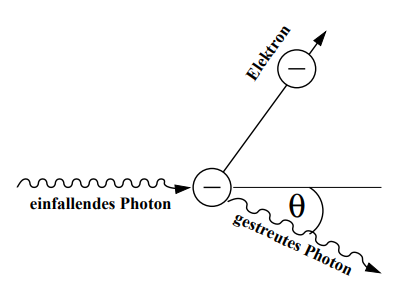
\includegraphics[width=0.5\textwidth]{bilder/comptonstreuung.png}
  \caption{Skizze des Streuvorgangs \cite{skript3}.}
  \label{fig:comptonstreuungskizze}
\end{figure}
\subsection{Erzeugung von Röntgenstrahlung}
Aus einer Glühkatode werden durch eine Heizspannung Elektronen gelöst, welche in einer evakuirten Röhre auf eine Anode beschleunigt werden. Beim Auftreffen auf die Anode werden
zwei Arten von Strahlung erzeugt (siehe \cite{skript4}). Zum einen die Bremsstrahlung, durch das Abbremsen der Elektronen an den Atomen des Anodenmaterials, und die charakteristische Strahlung, durch die
Anregung von Elektronen in den Atomen der Anode und das anschließende zurückfallen auf ein niedrigeres Energieniveau. Die abgegebene Energie der Elektronen bei der Abbremsung erhält das ausgesendete Photon, da die Elektronen 
allerdings nicht immer ihre ganze Energie abgeben entsteht ein kontinuirliches Spektrum. Das charakteristische Spektrum besteht dabei aufgrund der diskreten Energieniveaus des Anodenmaterials aus scharfen Linien. Die Energie dieser 
Quanten entspricht genau der Differenz der Energieniveaus beim \enquote{zurückfallen} der Elektronen.
\subsection{Transmission und Absorption}
Transmission beschreibt die Durchlässigkeit einer Strahlung durch ein bestimmtes Medium. Die Transmission eines Stoffes nimmt mit steigender 
Energie und somit sinkender Wellenlänge zu. Daraus folgt sofort, dass die durch den Compton-Effekt verschobene Strahlung schlechter transmittiert als die
höherenergetische Strahlung vor der Streuung.
\\
Ein Teil der Strahlung wird vom Stoff absorbiert und hier gilt das Delamber´sche Gesetz, welches die Abnahme der Strahlungsintensität beschreibt.
\begin{equation}
\label{eqn:delamber}
I = I_{0} \cdot \text{exp}^{-\mu d}
\end{equation}
Dabei ist $d$ die Dicke des Materials, $I_{0}$ die Intensität zu Beginn und $\mu$ der Absorptionskoeffizient.
\\
Die Wechselwirkung von Strahlung mit Materie ist im Allgemeinen nicht immer auf einen bestimmten Prozess limitiert. Das bedeutet neben der Compton-Streuung kommt
es ebenfalls zum Photoeffekt bei dem die Photonen die Elektronen im Material herauslösen. Die Paarbildung zu einem Elektron-Positron Paar spielt ebenfalls eine Rolle.
Der Absorptionskoeffizient sollte also bei einer allgemeinen Betrachtung von den genanten Prozessen abhängig sein.
\begin{equation*}
\mu = \mu_{\text{compton}} + \mu_{\text{photoeffekt}} + \mu_{\text{paarbildung}}
\end{equation*}

\subsection{Bragg-Bedingung}
Die Energie und damit die Wellenlänge lässt sich durch eine Reflexion an einem ausgewählten Kristall bestimmen. Hierbei fällt die 
zu untersuchende Strahlung auf das dreidimensionales Gitter und wird dort gebeugt. Durch die entstehenden Interferenzmuster und damit verbundenen Bedingungen lässt sich
die Wellenlänge ermitteln. Diese Formulierung wird Bragg-Bedinung genannt (siehe \cite{skript4}).
\begin{equation}
\label{eqn:lambda}
2 d \text{sin}(\theta) =  n \lambda \quad | n \in \mathbb{N}
\end{equation}
Hierbei ist $n$ ein ganze natürliche Zahl und steht für die Beugungsordnung. Dies folgt aus der Voraussetzung für den Gangunterschied bei konstruktive Interferenz
. Die Gitterkonstante $d$ ist dabei abhängig vom verwendeten Kristall.
Im folgenden Versuch wurde ein LiF- Kristall mit einer Gitterkonstanten $d$ von
\begin{equation}
d = \SI{201.4e-12}{\meter}
\end{equation}
verwendet.
Die Gleichung \eqref{eqn:lambda} gibt allerdings auch Aufschluss über den Winkel $\theta$ durch Umstellen zu.
\begin{equation}
\label{eqn:winkelmitlambda}
\theta = \text{arcsin}\left(\frac{n \cdot \lambda}{2 \cdot d}\right)
\end{equation}
Die Energie ergibt sich durch Einsetzen der Gleichung \eqref{eqn:lambda} in \eqref{eqn:photoneneq}.
\begin{equation}
    \label{eqn:braggEnergy}
    E = n \cdot \frac{h c}{2 d \sin (\theta)}
\end{equation}
Für die Berechnung der Transmission ist es meist notwendig bei Verwendung eines Geiger-Müllerzählrohrs eine Totzeitkorrektur durchzuführen.
Der korrigierte Wert der Zählraten kann dabei geschrieben werden als.
\begin{equation}
\label{eqn:totzeit}
I = \frac{N}{1 - \tau \cdot N}
\end{equation}
Das verwendete Geiger-Müllerzählrohr in der Versuchsdurchführung hat eine Totzeit von $\tau = \SI{90}{\micro\second}$.
Die Transmission $T$ erhält man anschließend durch eine Betrachtung der Strahlungszählratenverhältnisse mit und ohne Absorber.
\begin{equation}
\label{eqn:wichtig}
T = \frac{I_{\text{absorber}}}{I_{\text{ohne}}}
\end{equation}

